\documentclass{article}

% if you need to pass options to natbib, use, e.g.:
%     \PassOptionsToPackage{numbers, compress}{natbib}
% before loading neurips_2019

% ready for submission
% \usepackage{neurips_2019}

% to compile a preprint version, e.g., for submission to arXiv, add add the
% [preprint] option:
%     \usepackage[preprint]{neurips_2019}

% to compile a camera-ready version, add the [final] option, e.g.:
     \usepackage[final]{neurips_2019}

% to avoid loading the natbib package, add option nonatbib:
%     \usepackage[nonatbib]{neurips_2019}

\usepackage[utf8]{inputenc} % allow utf-8 input
\usepackage[T1]{fontenc}    % use 8-bit T1 fonts
\usepackage{hyperref}       % hyperlinks
\usepackage{url}            % simple URL typesetting
\usepackage{booktabs}       % professional-quality tables
\usepackage{amsfonts}       % blackboard math symbols
\usepackage{nicefrac}       % compact symbols for 1/2, etc.
\usepackage{microtype}      % microtypography
\usepackage{graphicx}       % display figure
\usepackage{hyperref}       % clickable links

\title{Midterm Report for 11-785}

% The \author macro works with any number of authors. There are two commands
% used to separate the names and addresses of multiple authors: \And and \AND.
%
% Using \And between authors leaves it to LaTeX to determine where to break the
% lines. Using \AND forces a line break at that point. So, if LaTeX puts 3 of 4
% authors names on the first line, and the last on the second line, try using

\author{%
  Ke Xu \\
  Electrical and Computing Engineering\\
  Carnegie Mellon University\\
  Pittsburgh, PA 15213 \\
  \texttt{kxu2@andrew.cmu.edu} \\

  \And
  Nicky Nocerino \\
  Electrical and Computing Engineering\\
  Carnegie Mellon University\\
  Pittsburgh, PA 15213 \\
  \texttt{nnocerin@andrew.cmu.edu} \\

  \And
  Yilin Wang \\
  Civil and Environment Engineering\\
  Carnegie Mellon University\\
  Pittsburgh, PA 15213 \\
  \texttt{yilinw2@andrew.cmu.edu} \\

  \And
  Zhufeng Fan \\
  Civil and Environment Engineering\\
  Carnegie Mellon University\\
  Pittsburgh, PA 15213 \\
  \texttt{zhufengf@andrew.cmu.edu} \\
  % examples of more authors
  % \And
  % Coauthor \\
  % Affiliation \\
  % Address \\
  % \texttt{email} \\
  % \AND
  % Coauthor \\
  % Affiliation \\
  % Address \\
  % \texttt{email} \\
  % \And
  % Coauthor \\
  % Affiliation \\
  % Address \\
  % \texttt{email} \\
  % \And
  % Coauthor \\
  % Affiliation \\
  % Address \\
  % \texttt{email} \\
}

\begin{document}

\maketitle
%%%%%%%%%%%%%%%%%%%%%%% Abstract %%%%%%%%%%%%%%%%%%%%
\begin{abstract}

Energy consumption is a popular topic with an increasing concern of global climate change and green gas emission. Saving energying has been widely admitted as an inevitable action for the people throughout the world. Since computer intelligence are expected to perform more sensitive than human beings, deep learning algorithms especially data pattern detection has been applied to optimize energy plan for the system operators. However, a significant amount of approaches based on supervised machine
learning models that require (big) labelled data-set. In this project, we are expected to analyze the energy using data and detect the abnormality phenomena based on an optimized Auto-encoder model. Firstly, we will implement and replicate experimental results. Secondly, we will try to improve the performance of the model by replacing Bi-LSTM with Transformer. Finally, we will implement a multi-class framework based on previous model to discriminate between different anomalies using the latent
features in the z-space. Now we have finished two baseline experiments(MLP and LSTM auto-encoder). They have good performance on the mnist dataset. We can see a very clear loss threshold between the normal and abnormal data.


\end{abstract}

%%%%%%%%%%%%%%%%%%%%%%% Introduction %%%%%%%%%%%%%%%%%%%%
\section{Introduction}
The time series energy data are widely used right now. The data makes it possible to develop machine learning algorithms that can anaylyse and monitor the data collected and detect anomalous behaviour in the energy field, which contributes to improving the safety of the high power systems. The problem of finding patterns in data that do not conform to expected or normal behaviour is often referred to as Anomaly Detection. Since the mid-1990s, many computer science researchers have been working on how to automatically detect anomalies and many methods have been proposed. In particular, recently reserachers have successfully built some robust deep learning models with large dataset to detect anomalies. 

However, a significant amount of these approaches are based on supervised machine learning models that require (big) labelled datasets to be trained. Furthermore, some of the proposed methods do not consider the sequential nature of the data by assuming it is independent in time. To address the above issues, Joao Pereira and Margarida Silveira proposed a method called Variational Recurrent Autoencoders with Attention \cite{AuthorJM}, which uses time series data to train an unsupervised model. 

Our project is based on Joao Pereira and Margarida Silveira's work. First, we will implement their model and replicate their experimental results. Then we will try to improve the performance of the model by replacing Bi-LSTM with Transformer. Finally, we will implement a multi-class framework based on our previous model to discriminate between different anomalies using the latent features in the z-space.

%%%%%%%%%%%%%%%%%%%%%%% Literature Review %%%%%%%%%%%%%%%%%%%%
\section{Literature Review}
In recent years, various machine learning methods have been applied widely to automate the process monitoring and fault diagnosis. Artificial neural networks are popular due to a simplicity in logic and a powerful ability to deal with nonlinear problems such as abnormally detection. Typical supervised learning method with various build-in structures, for example, multi-layer perceptron (MLP) \cite{AuthorSI}, learning vector quantization networks (LVQ), were used to detect simple patterns such as shift, trend, cycle etc. With a further development of the network structure, hybrid model with a combination of models come into appear.

\subsection{Abnormally detection}
Abnormally detection has been widely used on system control and management. Potes and Cristhian development of an algorithm to classify normal/abnormal heart sounds from the observation dataset on human bodies. A total of 124 time-frequency features were extracted from the phonocardiogram (PCG) which is used as an input of a convolutional neural network (CNN) based on an ensemble of classifiers combining the outputs of AdaBoost. \cite{AuthorPotes} Du and Min (2017), proposed a Long Short-Term
Memory (LSTM), to model a system log as a natural language sequence. With and automatic learning from log patterns, it allowed the algorithm to detect anomalies when log patterns deviate from the model trained from log data under normal execution. \cite{AuthorDu}

\subsection{Auto-encoder (AE) and Auto-decoder (AD) network}
With addressing a large scale of data and high-dimensional level of learning, autoencoder (AE) makes its way into health monitoring \cite{AuthorRZ}, fault diagnosis AE models could learn representative features from raw data by reconstructing input data from an artificial corruption. For years, AE models have been widely used on diverse fields to deal with the practical problem. Chen, Min, et al (2017), proposes a convolutional autoencoder deep learning framework to support unsupervised image
features learning for lung module with a small amount of labeled data for efficient feature learning. Kamper and Herman (2015), proposed an unsupervised neural network feature extractor without resources in zero-resource settings. They achieved a two-third of relative improvement with the feature extractor in a word discrimination task. \cite{AuthorKa} Fan and Cheng (2018) investigates the potential of autoencoders in detecting anomalies in building energy data. Specific methods have been
designed to evaluate the autoencoder performance, the results can be used as foundation for building professionals to develop advanced tools for anomaly detection. 

%%%%%%%%%%%%%%%%%%%%%%% Dataset %%%%%%%%%%%%%%%%%%%%
\section{Dataset}
\subsection{MNIST}
The "mnist" dataset is a public image database of handwritten digits that is commonly used for training various image processing systems. Our goal is to test the performances of our baseline anomaly detection model by feeding the images from mnist dataset.
\url{https://en.wikipedia.org/wiki/MNIST_database}

This dataset is very small. It won't take a long time to trian our model and we can easily add noise to the test images to create abnormal data. That's why we choose to use mnist for our baseline models. Firstly, a dataset with noises is supposed to be generated. We selected 1000 samples from the test data and added random noise. Gaussian noise is applied in this case. Then we conbine the 1000 abnormal data with the remaining 9000 clean data to form an abnormal test dataset. We will use the
train data of mnist dataset to train our model and abnormal test data to test whether our autoencoders can successfully detect the abnormality.

\subsection{EMHIRES dataset}
EMHIRES is the first publically available European solar power generation dataset derived from meteorological sources that is available up to NUTS-2 level. It was generated applying the PVGIS model to capture local geographical information to generate meteorologically derived solar power time series at high temporal and spatial resolution. This allows for a better understanding of the solar resource at the precise location of wind farms.

EMHIRES provides RES-E generation time series for the EU-28 and neighbouring countries. The solar power time series are released at hourly granularity and at different aggregation levels: by country, power market bidding zone, and by the European Nomenclature of territorial units for statistics (NUTS) defined by EUROSTAT; in particular, by NUTS 1 and NUTS 2 level. The time series provided by bidding zones include special aggregations to reflect the power market reality where this deviates from political or territorial boundaries.

The overall scope of EMHIRES is to allow users to assess the impact of meteorological and climate variability on the generation of solar power in Europe and not to mime the actual evolution of solar power production in the latest decades. For this reason, the hourly solar power generation time series are released for meteorological conditions of the years 1986-2015 (30 years) without considering any changes in the solar installed capacity. Both the Country level and NTUS level data contain
262,968 hourly time steps, from 1986/1/1 00:00 to 2015/12/31 23:00. The number of samples are shown in Table 1.

\begin{table}
  \caption{Raw inspection data records count by inspection year}
  \label{obd data}
  \centering
  \begin{tabular}{cccc}
    \toprule
    \multicolumn{4}{c}{Samples}                   \\
    \cmidrule(r){1-4}
    Year & Records & Year & Records      \\
    \midrule
    2000 & $3,000,804$ & 2003 & $3,151,591$     \\
    2001 & $3,057,150$ & 2004 & $5,562,887$       \\
    2002 & $3,103,306$ & 2005 & $5,611,680$      \\
    \bottomrule
  \end{tabular}
\end{table}


%%%%%%%%%%%%%%%%%%%%%%% Evaluation Matrix %%%%%%%%%%%%%%%%%%%%
\section{Evaluation Matrix}
Since we only use the clean data to train our models, abnormal test data will have a larger loss than the clean test data. So we can select a threshold in the loss gap to determine whether the data is clean or abnormal. Besides, we will use confusion matrix to evaluate our models.

\subsection{Confusion Matrix}
Confusion matrix, also known as an error matrix, is a specific table layout that allows visualization of the performance of an algorithm. A classic confusion matrix is a $2\times 2$ table with four attributes, each of which are listed as TP (True Positive), TN (True Negative), FP(False Positive) and FN(False Negative). Table 2 shows the detailed definition of the matrix. (see the url: \url{https://en.wikipedia.org/wiki/Confusion_matrix})

Considering the expected results of anomaly detection is binary, choosing confusion matrix as the evaluation Matrix would be a good way to visualize the performance of the detection model neat and tidy. 

\begin{table}
  \caption{Confusion Matrix of supervised learning}
  \label{obd data}
  \centering
  \begin{tabular}{cccc}
    \toprule
    \multicolumn{3}{c}{True Condition}                   \\
    \cmidrule(r){1-3}
    & Condition positive & Condition negative      \\
    \midrule
    Predicted positive & $TP$ & $FP$     \\
    Predicted negative & $FN$ & $TN$       \\
    \bottomrule
  \end{tabular}
\end{table}


%%%%%%%%%%%%%%%%%%%%%%% Model Baseline %%%%%%%%%%%%%%%%%%%%
\section{Experimental Baseline}
Though the paper says that the autoencoder can successfully detect abnormality, we want to test whether and how well it works. So we built a MPL autoencoder to test the performance of the autoencoder and whether our evalution metics works well. Next we built a LSTM autoEncoder to capture the high-level information of input data instead of MLP, because our final model will be based on RNN, which can help us to caputer the features of the time-series data. We want to test whether RNN
architectures works well in the autoencoder. We use our own abnormal mnist dataset on both models. Here is the link of our project:\href{https://github.com/Dylan-Wyl10/11-785-20F-project}{11785 project}

\subsection{MLP-Baseline}
Under the context of baseline Dataset (MNIST), the encoder and decoder architectures of MLP, built using Pytorch: 
\begin{itemize}
\item Decoder: \\
Linear (28*28, 128) + ReLU \\
Linear (128, 64) + ReLU \\
Linear (64, 12) + ReLU \\
Linear (12, 3) \\
\item Encoder: \\
Linear (3, 12) + ReLU \\
Linear (12, 64) + ReLU \\
Linear (64, 128) + ReLU \\
Linear (128, 28*28) + ReLU \\
Loss: MSE loss \\
\end{itemize}
Optimizer: SGD, learning rate=1e-2, weight decay=1e-5, momentum=0.9, train 3 epochs.\\
We choose this model because it could map image data into a relatively small latent space using few linear layers and hidden neurons, which could made training fast and require not too many parameters. 
However, the MLP model is not able to generate latent space for time-series data without context augmentation. So we also built a Bi-LSTM AutoEncoder, which include a LSTM layer and a Linear layer in both encoder and decoder.  

\subsection{LSTM-Baseline}
Under the context of baseline Dataset (MNIST), the encoder and decoder architectures of Bi-LSTM, built using Pytorch: 
\begin{itemize}
\item Decoder: \\
LSTM (28, 256, 3)  \\
Linear (512, 12) \\
\item Encoder: \\
LSTM (12, 256, 3)  \\
Linear (512, 28) \\
Loss: MSE loss \\
\end{itemize}
Optimizer: SGD, learning rate=1e-2, weight decay=1e-5, momentum=0.9, train 3 epochs.\\
Compared to the MLP-Baseline model, Bi-LSTM gives us a larger gap between the loss of clean and abnormal test data, which means it can discriminate the clean and abnormal data better.

\subsection{Assumptions}
Several assumptions have been made to narrow down the scope of the baseline experiment. The main objectives is to test the model, thus the assumptions are not considering the closeness between model and real world.
The assumptions are as below:
\begin{itemize}
    \item Images with Gaussian noise can be considered as abnormal data.
    \item In this experiment, we will use a fixed range of threshold as a classifier to distinguish the normal data and anomaly data. In other word, the threshold is expected to perfectly classify the clean and abnormal data. 
\end{itemize}

\subsection{Caveats}
The concept of abnormality is very hard to define and have a lot of different forms. Detecting other abnormalities may not have such a good performance compared to detecting tha abnormality of adding Gaussian noise. 

\subsection{Conclusion}
After a training with mnist training data and test the model with generated dataset that contains abnormal. We can conclude a classification result with the distribution of losses. Figure 1 shows the distributions of the loss of test data. Besides, the confusion matrix when threshold is equal to 0.3 is shown in Table 3.
For those images with noises, the losses are distributed around 0.35 while images without noises have a loss cluster around 0.1. In this case, a range between 2.2 to 3.0 would be a perfect threshold for setting up the classifier. However, this result can only
prove the feasibility of the baseline model but the value itself could be weak since the assumptions have narrowed down a lot. 

In short, our baseline models have good performance on mnist dataset. But we need to extend it to the EMHIRES dataset. It requires a complext RNN with Attention, which we are currently working on. Besides, a fixed threshold may not be a good idea. We will try to come up with a stable way to determine whether data are abnormal or not. 

\begin{figure}[!t]
    \centering
    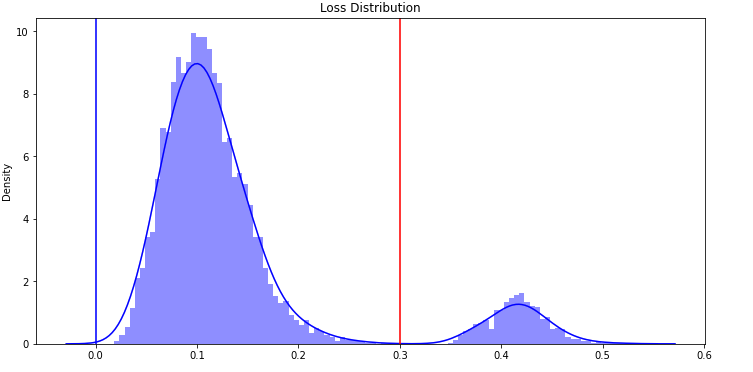
\includegraphics[width=0.7\textwidth]{images/Baseline result.png}
    \caption{Classification distributions on baseline experiment}
\end{figure}


\begin{table}
  \caption{Confusion Matrix of supervised learning}
  \label{obd data}
  \centering
  \begin{tabular}{cccc}
    \toprule
    \multicolumn{3}{c}{True Condition}                   \\
    \cmidrule(r){1-3}
    & Condition positive & Condition negative      \\
    \midrule
    Predicted positive & $9000$ & $0$     \\
    Predicted negative & $0$ & $1000$       \\
    \bottomrule
  \end{tabular}
\end{table}

%%%%%%%%%%%%%%%%%%%%%%% Current experiments %%%%%%%%%%%%%%%%%%%%
\section{Current experiments}
Now we are working on implementing Variational Recurrent Autoencoders with Attention \cite{AuthorJM} proposed by Joao Pereira and Margarida Silveira because we need a bi-direction LSTM with Attention to better capture the high-level feature of input data in EMHIRES dataset. We will replicate the experiment results in the paper using the EMHIRES dataset. The architecture of the model is shown in Figure 2. 

\subsection{Assumptions}
The assumptions for our current experiments are as below:

\begin{itemize}
\item We will still use a fixed range of threshold as a classifier to distinguish the normal data and anomaly data. In other word, the threshold is expected to perfectly classify the clean and abnormal data. However if it doensn't work well, we will consider using a variable threshold.

\item Our EMHIRES training data are clean enough. Some outliers in the training data won't affect the training results of our autoencoder model.

\end{itemize}
\begin{figure}[!t]
    \centering
    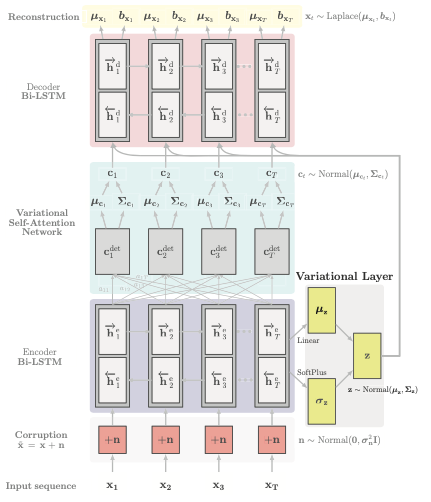
\includegraphics[width=0.7\textwidth]{images/BiLSTM.png}
    \caption{Variational Bi-LSTM Autoencoder with Variational Self-Attention.}
\end{figure}

%%%%%%%%%%%%%%%%%%%%%%% Methods %%%%%%%%%%%%%%%%%%%%
\section{Future Plan}

\subsection{Planned Experiment}
In the following weeks, we will Improve the performance of the model by replacing Bi-LSTM with Transformer. Finally, we will implement a multi-class framework based on our previous model to discriminate between different anomalies using the latent features in the z-space.

\subsection{Work Division}
The division of the work is showed below. For most of the work in this project, we will work together as a team.
The work division of the mid-term:
\begin{itemize}
    \item Dataset implementation: Ke XU and Zhufeng Fan
    \item LSTM baseline model implementation: Nicky Nocerino
    \item MLP baseline model implementation: Ke XU
    \item Proposal and midterm report: Yilin Wang, Ke XU, Zhufeng Fan, Nicky Nocerino
    \item Code organization and maintenance: Ke XU and Yilin Wang
\end{itemize}
In the coming weeks, our team will work on the real dataset and train the final model. The division is showed below:
\begin{itemize}
    \item Real data preparation and pre-processing: Zhufeng Fan, Ke XU
    \item Model implementation: Nicky Nocerino, Ke Xu, Yilin Wang
    \item Code maintenance: Yilin Wang, Ke Xu 
\end{itemize}

\subsection{Timeline}
The proposed timeline is as followed:
\begin{itemize}
    \item 
        11/17: Complete the implementation of current experiment.
    \item
        11/23: Replace Bi-LSTM with Transformer.
    \item
        11/29: Build a multi-class framework to dicriminate diffrent anomalies.
    \item
        12/02: Complete all the improvement of our model and debugging .
    \item
        12/04: Write the final report.
    \item 
        12/05: Prepare the slides for the project video.
    \item
        12/06: Recording the project video.
\end{itemize}

{
\bibliographystyle{unsrt}
\bibliography{egbib}
}

\end{document}
